\sectionquestion{Na\"{i}ve Bayes}

\begin{parts}

\part[2] \textbf{Math:} Suppose you are trying to train a Gaussian Na\"{i}ve Bayes model for multi-class classification: you have $D$ real-valued features and your label can be one of $C$ possible classes. \emph{Assume you are learning the means and variances from the training dataset}. Including the distribution over the label, how many parameters will you need to learn? 
\begin{tcolorbox}[fit,height=1.5cm, width=4.5cm, blank, borderline={1pt}{-2pt}]
    \begin{soln}
        $2DC+C-1$
        TODO: The early make-ups might have been counting only variances, so we'll need to give credit for those students only.
    \end{soln}
\end{tcolorbox}
\begin{qauthor}
    Henry
\end{qauthor}

\part For the following questions, use the toy dataset for heart disease prediction from lecture:

\begin{center}
\begin{tabular}{cccc}
    \toprule
    $x_1$: Family History & $x_2$: Blood Pressure & $x_3$: Cholesterol & $y$: Heart Disease?  \\
    \midrule
    Yes & Low & Normal & No \\
    No & Medium & Normal & No \\
    No & Low & Abnormal & Yes \\
    Yes & Medium & Normal & Yes \\
    Yes & High & Abnormal & Yes \\
    \bottomrule
\end{tabular}
\end{center}

\begin{subparts}
    \subpart[1] \textbf{Numerical Answer:} What is the MLE for $P(y=\textrm{Yes})$?
    \begin{tcolorbox}[fit,height=1.5cm, width=3cm, blank, borderline={1pt}{-2pt}]
        \begin{soln}
            $\frac{3}{5}$
        \end{soln}
    \end{tcolorbox}
        
    \subpart[1] \textbf{Numerical Answer:} Under the Na\"{i}ve Bayes assumption, what is the MLE for $P(x_1=\textrm{No} \mid y=\textrm{Yes})$?
    \begin{tcolorbox}[fit,height=1.5cm, width=3cm, blank, borderline={1pt}{-2pt}]
        \begin{soln}
            $\frac{1}{3}$
        \end{soln}
    \end{tcolorbox}
        
    \subpart[1] \textbf{Numerical Answer:} Under the Na\"{i}ve Bayes assumption, what is the MLE for $P(x_3=\textrm{Normal} \mid y=\textrm{No})$?
    \begin{tcolorbox}[fit,height=1.5cm, width=3cm, blank, borderline={1pt}{-2pt}]
        \begin{soln}
            $1$
        \end{soln}
    \end{tcolorbox}

\newpage
    \subpart[2] \textbf{Select one:} Suppose you train a Na\"{i}ve Bayes classifier using the training dataset above. How would your classifier classify a new patient with the following feature vector: [No, Low, Normal]? \textbf{For full credit, you must show your work in the space provided.}
    \begin{checkboxes}
        \choice Yes
        \choice No
        \choice Yes and No are equally likely
    \end{checkboxes}
    \begin{tcolorbox}[fit,height=6cm, width=15cm, blank, borderline={1pt}{-2pt}]
        \begin{soln}
            No, for each of the given features, the probability given No dominates the probability given Yes
        \end{soln}
    \end{tcolorbox}
\end{subparts}
\begin{qauthor}
    Henry
\end{qauthor}

\part Suppose you have a dataset $\mathcal{D}$ for binary classification that consists of $D$ binary features: and you fit a Na\"{i}ve Bayes classifier to the dataset using MLE to set the parameters; let this classifier be denoted by $C$. 
\begin{subparts}
    \subpart[2] \textbf{Short Answer:} Using the same dataset, suppose you fit another Na\"{i}ve Bayes classifier, this time using MAP to set the parameters by putting Beta priors over each of the feature distributions; let this classifier be denoted by $C^*$. Can $C$ and $C^*$ ever make different predictions for some unseen query data point $x$? Briefly justify your answer in 2-3 concise sentences. 
    \fillwithlines{9em}
    \begin{soln}
        Yes; as an example, suppose some parameters of $C$ were set $0$. $C^*$ cannot have any parameters equal to $0$ so it is entirely possible for the predictions to change. 
    \end{soln}

    \newpage
    \subpart[2] \textbf{Short Answer:} Now suppose you create a new dataset $\mathcal{D}'$ by duplicating \emph{all} of the data points in $\mathcal{D}$ and you fit a Na\"{i}ve Bayes classifier to $\mathcal{D}'$, reverting back to MLE to set the parameters; let this new classifier be denoted by $C'$. Can $C$ and $C'$ ever make different predictions for some unseen query data point $x$? Briefly justify your answer in 2-3 concise sentences. 
    \fillwithlines{9em}
    \begin{soln}
        No; for each feature, duplicating the dataset will not change the fraction of data points where that feature has value 1 for either label. Thus the MLE of all the parameters will be the same for both $C$ and $C'$ so the two classifiers will behave identically. 
    \end{soln}
\end{subparts}

% \part Consider learning a 2D Gaussian Naive Bayes model for binary classification on the dataset shown below.

%     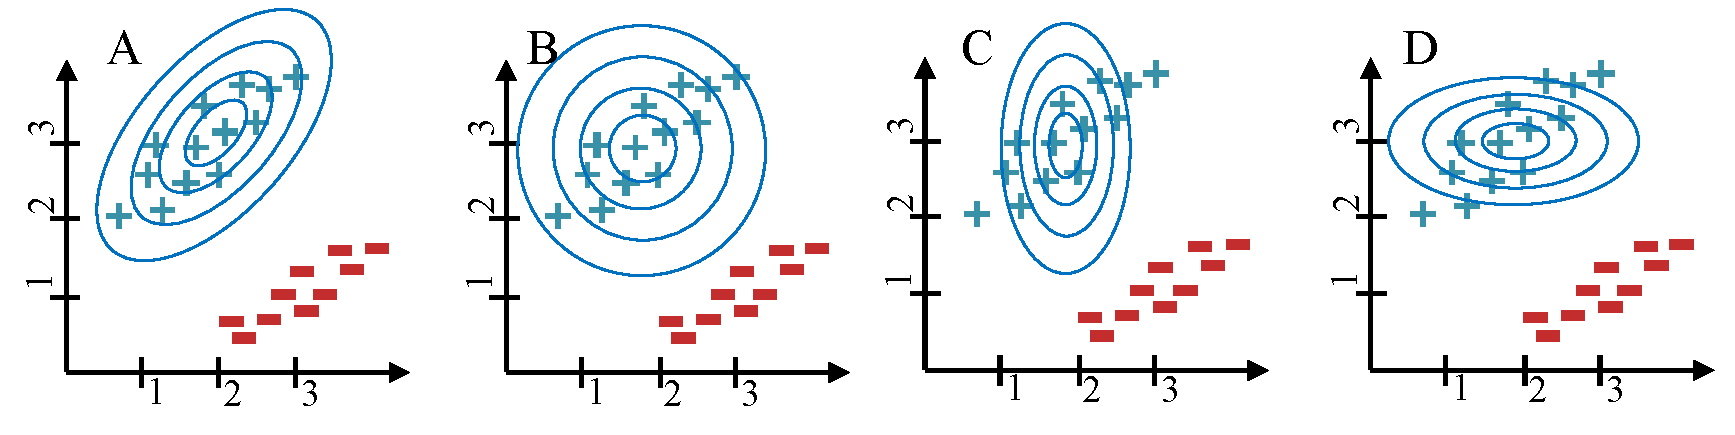
\includegraphics[scale=0.5]{figures/contours.pdf}

%     \begin{subparts}
    
%     \subpart[1] \textbf{Select one:} Assuming the means and variances are all learned without parameter tying or fixing to a constant, which of the contour plots describing the density $f(x_1, x_2 \mid y=1)$ best describes what would be learned?
%     \begin{checkboxes}
%      \choice A
%      \choice B
%      \choice C
%      \choice D
%     \end{checkboxes}
%     \begin{soln}
%     B
%     \end{soln}

%     \subpart[1] \textbf{Select one:} Assuming the means are learned but the variances are fixed to 1.0, , which of the contour plots describing the density $f(x_1, x_2 \mid y=1)$ best describes what would be learned?
%     \begin{checkboxes}
%      \choice A
%      \choice B
%      \choice C
%      \choice D
%     \end{checkboxes}
%     \begin{soln}
%     B
%     \end{soln}

%     \end{subparts}
%     \begin{qauthor}
%     Matt
%     \end{qauthor}

\begin{comment}
\part Mr. Chameleon takes lots of selfies and decides to build a classifier to predict a label $y$ indicating whether he looks more like a flamingo or a brown bear in his latest selfie. He designs two features: $x_1$ stores the \% of pink pixels binned into three bins (0-32, 33-65, 66-100), $x_2$ stores the \% of brown pixels binned into two bins (0-49, 50-100). 

\begin{center}
\begin{tabular}{ccc}
    \toprule
    $x_1$ & $x_2$ & $y$  \\
    \midrule
    66-100 & 0-49 & bear \\
    66-100 & 0-49 & flamingo \\
    33-65 & 0-49 & flamingo \\
    33-65 & 50-100 & bear \\
    0-32 & 50-100 & bear \\
    \bottomrule
\end{tabular}
\end{center}

%The feature design leaves Mr. Chameleon feeling a bit mixed-up, since he can use neither Bernoulli Naive Bayes, nor Multinomial Naive Bayes. He combines the two into a new model, Mixed-up Naive Bayes, that uses a Multinomial event model for $p(x_1 \mid y)$, a Bernoulli event model for $p(x_2 \mid y)$, and a separate Bernoulli for $p(y)$.
The feature design leads Mr. Chameleon to use a Multinomial Naive Bayes model.
%, but he's a bit mixed-up about how to train the model. Help him answer these questions.

    \begin{subparts}

    \subpart[1] \textbf{Numerical answer:} How many parameters does this Multinomial Naive Bayes model have for the given dataset?
        \begin{tcolorbox}[fit,height=1cm, width=2cm, blank, borderline={1pt}{-2pt}]
        %solution
        \end{tcolorbox}
        \begin{soln}
        7 =  4 for $x_1$, 2 for $x_2$, 1 for $y$
        \end{soln}

    \subpart[1] \textbf{Numerical answer:} What is the MLE for $p(y = \text{flamingo})$?
        \begin{tcolorbox}[fit,height=1cm, width=2cm, blank, borderline={1pt}{-2pt}]
        %solution
        \end{tcolorbox}
        \begin{soln}
        2/5
        \end{soln}
    
    \subpart[1] \textbf{Numerical answer:} What is the MLE for $p(x_1 = \text{0-32} \mid y = \text{flamingo})$?
        \begin{tcolorbox}[fit,height=1cm, width=2cm, blank, borderline={1pt}{-2pt}]
        %solution
        \end{tcolorbox}
        \begin{soln}
        0
        \end{soln}
        
    \subpart[1] \textbf{Numerical answer:} What is the MLE for $p(x_1 = \text{0-32} \mid y = \text{bear})$?
        \begin{tcolorbox}[fit,height=1cm, width=2cm, blank, borderline={1pt}{-2pt}]
        %solution
        \end{tcolorbox}
        \begin{soln}
        1/3
        \end{soln}

    \subpart[1] \textbf{Numerical answer:} What is the MLE for $p(x_2 = \text{0-49} \mid y = \text{bear})$?
        \begin{tcolorbox}[fit,height=1cm, width=2cm, blank, borderline={1pt}{-2pt}]
        %solution
        \end{tcolorbox}
        \begin{soln}
        1/3
        \end{soln}
    
    % \uplevel{
    % Suppose Mr. Chameleon collects an additional one hundred training examples and learns the following parameters of the model.

    % \begin{align*}
    %     & p(y = \text{flamingo}) = 3/10 \\
    %     & p(y = \text{bear}) = 7/10 \\
    %     & p(x_1 = \text{0-32} \mid y = \text{flamingo}) = 3/10 \\
    %     & p(x_2 \text{0-49 \mid y = \text{bear}) = 7/10 \\
    % \end{align*}
    
    % }
                
    % \subpart[1] \textbf{Select one:} After completing his maximum likelihood estimation of all the parameters, Mr. Chameleon takes a test selfie and mistakenly\footnote{Kindly ignore Mr. Chameleon's error and proceed with the features he has given, even though they imply a total percentage of pink and brown pixels greater then 100\%.} writes down the following features $x1 = \text{66-100}$ and $x_2 = \text{50-100}$. How would his Mixed-up Naive Bayes model classify this test instance? 
    %     \begin{checkboxes}
    %      \choice flamingo
    %      \choice bear
    %      \choice tie in probability
    %     \end{checkboxes}
    %     \begin{soln}
    %     Both $p(y = \text{flamingo} \mid \xv)$ and $p(y = \text{bear} \mid \xv)$ have zero probability. It's a tie.
    %     \end{soln}

       
    \subpart[2] \textbf{Select one:} After completing his maximum likelihood estimation of all the parameters, Mr. Chameleon takes a test selfie and writes down the features of this test instance as $x_1 = \text{66-100}$ and $x_2 = \text{0-49}$. How would his model classify this test instance? 
        \begin{checkboxes}
         \choice flamingo
         \choice bear
         \choice tie in probability
        \end{checkboxes}
        \begin{soln}
        flamingo: 1/2 * 1/2 * 2/5
        bear: 1/3 * 1/3 * 3/5
        \end{soln}
        
    \end{subparts}
    \begin{qauthor}
    Matt
    \end{qauthor}

\part[1] \textbf{Short answer:} Give one example in which MAP estimation might be preferred over MLE when training a Naive Bayes classifier for classifying whether a document was authored by Henry David Thoreau or Rachel Carson using word counts as features.
    \fillwithlines{6em}
    \begin{soln} 

    If there are words that only appear with one label in the training data, MLE would give zero probability to the other label whenever that word is present, but MAP might not. 

    If you know one author is more inclined to write about one topic than the other author (e.g. marine biology for Rachel Carson and the other about civil disobediance for Henry David Thoreau), imposing a prior over those topic oriented words could help.

    If you don't have much training data, but you have world knowledge about the authors.
    
    Very general answer that is sort of correct, but doesn't address the specific case of Naive Bayes for authorship classification: MAP estimation is preferred over other methods of estimation when there is some prior information available and the amount of available data is limited. It allows us to incorporate this prior information into our estimate. %\\
    %MAP estimation may not be appropriate when the prior information is unreliable or inconsistent with the observed data. 
    \end{soln}
    \begin{qauthor}
    Yash, MLE and MAP
    \end{qauthor}   
\end{comment}
\end{parts}